\documentclass{article}
% Change "article" to "report" to get rid of page number on title page
\usepackage{amsmath,amsfonts,amsthm,amssymb}
\usepackage{setspace}
\usepackage{Tabbing}
\usepackage{fancyhdr}
\usepackage{lastpage}
\usepackage{extramarks}
\usepackage{url}
\usepackage{chngpage}
\usepackage{longtable}
\usepackage{soul,color}
\usepackage{graphicx,float,wrapfig}
\usepackage{enumitem}
\usepackage{morefloats}
\usepackage{multirow}
\usepackage{multicol}
\usepackage{indentfirst}
\usepackage{lscape}
\usepackage{pdflscape}
\usepackage{natbib}
\usepackage[toc,page]{appendix}
\providecommand{\e}[1]{\ensuremath{\times 10^{#1} \times}}

% In case you need to adjust margins:
\topmargin=-0.45in      % used for overleaf
%\topmargin=0.25in      % used for mac
\evensidemargin=0in     %
\oddsidemargin=0in      %
\textwidth=6.5in        %
%\textheight=9.75in       % used for mac
\textheight=9.25in       % used for overleaf
\headsep=0.25in         %

% Homework Specific Information
\newcommand{\hmwkTitle}{Progress Report 1}
\newcommand{\hmwkDueDate}{Monday,\ September\  24,\ 2018}
\newcommand{\hmwkClass}{Final Project}
\newcommand{\hmwkClassTime}{CSE 597}
\newcommand{\hmwkAuthorName}{Yueze Tan}
\newcommand{\hmwkNames}{yut75}

% Setup the header and footer
\pagestyle{fancy}
\lhead{\hmwkNames}
\rhead{\hmwkClassTime: \hmwkTitle} 
\cfoot{Page\ \thepage\ of\ \pageref{LastPage}}
\renewcommand\headrulewidth{0.4pt}
\renewcommand\footrulewidth{0.4pt}

%%%%%%%%%%%%%%%%%%%%%%%%%%%%%%%%%%%%%%%%%%%%%%%%%%%%%%%%%%%%%
% Make title

\title{\vspace{2in}\textmd{\textbf{\hmwkClass:\ \hmwkTitle}} \\
\vspace{0.1in}\large{ \hmwkClassTime}\vspace{3in}}

\author{\textbf{\hmwkAuthorName} \\ \vspace{0.1in}
\hmwkDueDate }
\date{} % to take away today's date

%%%%%%%%%%%%%%%%%%%%%%%%%%%%%%%%%%%%%%%%%%%%%%%%%%%%%%%%%%%%%

\begin{document}
\begin{spacing}{1.1}
\maketitle

\newpage
\section*{Abstract}

Discussed in this report is the numerical approaches to solving of modified electrostatic Poisson equation with shielding effect that has a characteristic shielding length (known as Debye length). We first introduce the equation $(\nabla^2 - \lambda_D^{-2})\Phi =-\rho / \varepsilon$ along with its physical meanings, then describe the discretization method. Direct solver (partial-pivoting LU decomposition) and iterative solver (Jacobi method) are both introduced and compared.

\section{Problem of Interest}

The problem is related with solving the electrostatic equation in a system with free charges and shielding effects, typical examples of which would be plasma or electrolytes. From Boltzmann's distribution we can obtain the equation describing the shielded, or compensated field:
\[(\nabla^2 - \lambda_D^{-2})\Phi=-\frac{\rho}{\varepsilon},\]
in which $\Phi$ is the electric potential, $\rho$ is the charge density which is contributed by other effects than shielding, like charge density induced by inhomogeneous distribution of polarization in a dielectric matter, and $\varepsilon$ is permittivity of the system.

For free-moving charge is common in various physical systems, charge compensation and spontaneous shielding effect could be widely observed in different kinds of condensed systems. In order to get a more accurate solution in these systems, solving the electrostatic equation with Debye length term is a necessary step. The distribution of electric potential is an interested topic in various fields, like materials science, condensed matter physics and chemical engineering, where electrolytes are extensively discussed.

Other numerical methods could also be applied to solve this problem, as what could be done for many other different types of PDEs. One possible way is using finite-element method (FEM), in which we discretize the system into piecewise functions, and then transform the problem into a integration form:
\[\int_V\left[(\nabla^2-\lambda_D^{-2})\Phi+\frac{\rho}{\varepsilon}\right]v_i\;\mathrm{d}V=0,\]
in which $v_i$ is a set of specially chosen functions to simplify the integrations.

Or we can use fast Fourier transform (FFT) to solve this problem, by transforming the original field into Fourier spectrum and then solve the algebraic equation in the frequency domain:
\[(k_1^2+k_2^2+k_3^3-\lambda_D^{-2})\Phi^K=-\frac{\rho^K}{\varepsilon},\]
and by taking inverse FFT (IFFT) on the spectrum we can get the field in real space. Such a method has already been used to solve the conventional electrostatic problem in phase-field models, see \citep{li2002}.

It might be of the readers' interest that this problem has an analytical solution, which is based on its Green function:
\[ \Phi(\mathbf{r}) =
\int _V \frac{\rho(\mathbf{r'}) (\mathbf{r} - \mathbf{r'}) \exp(|\mathbf{r} - \mathbf{r'}| / \lambda_D)}{|\mathbf{r} - \mathbf{r'}|^3} \;\mathrm{d}^3 \mathbf{r'} +
\oint _{\partial V} \frac{\sigma(\mathbf{r'}) (\mathbf{r} - \mathbf{r'}) \exp(|\mathbf{r} - \mathbf{r'}| / \lambda_D)}{|\mathbf{r} - \mathbf{r'}|^3} \;\mathrm{d} S.\]
Basically, this solution is a modified version of the regular electrostatic solution for Poisson equation, but equipped with an exponentially decaying factor so the electric potential drops much faster, which is what we are expecting from a shielding effect.

However, carrying out such an integration is practically unfavourable for most cases, as the time consumption is not satisfying, and precision of numerical solution is also suspicious since the expression to be integrated is divergent at $\mathbf{r} = \mathbf{r'}$. Besides, for most cases the boundary condition is of Dirichlet's type, which means $\sigma(\mathbf{r'})$ is unknown on the boundary of the integrated region. Therefore, a numerical way of solving the original PDE is practically more favourable.

\subsection{Numerical Set-up}

We discretize the original system using finite difference method with a uniform meshgrid, so that for a field $f(x,y,z)$, its discretized form will be
\[f_{i,j,k}=f(i\Delta x, j\Delta y, k\Delta z).\]
Hereafter, we set the discretization step as $\Delta x = \Delta y = \Delta z = 1$ nm.
Using Taylor's expansion,
\[f(x+\Delta x) = f(x)+\frac{\partial f(x)}{\partial x}\Delta x+\frac{1}{2!}\frac{\partial ^2 f(x)}{\partial x^2} (\Delta x)^2+\dots ,\]
\[f(x-\Delta x) = f(x)-\frac{\partial f(x)}{\partial x}\Delta x+\frac{1}{2!}\frac{\partial ^2 f(x)}{\partial x^2} (\Delta x)^2-\dots .\]
By adding them up and deprecating terms higher than 3rd order, we have
\[\frac{\partial^2 f(x)}{\partial x^2}\approx\frac{f(x+\Delta x)+f(x-\Delta x)-2f(x)}{(\Delta x)^2}.\]
Therefore the original equation could now be discretized as
\[\frac{\Phi_{i+1,j,k}+\Phi_{i-1,j,k}-2\Phi_{i,j,k}}{(\Delta x)^2}+
\frac{\Phi_{i,j+1,k}+\Phi_{i,j-1,k}-2\Phi_{i,j,k}}{(\Delta y)^2}+
\frac{\Phi_{i,j,k+1}+\Phi_{i,j,k-1}-2\Phi_{i,j,k}}{(\Delta z)^2}-
\lambda_D^{-2}\Phi_{i,j,k}
=-\frac{\rho_{i,j,k}}{\varepsilon}.\]

By arranging the values of a field in a vector,
\[\mathbf{f}=\left[\begin{matrix}f_{0,0,0} \\ \vdots \\ f_{i-1,j,k} \\ f_{i,j,k} \\ f_{i+1,j,k} \\ \vdots \\ f_{i,j+1,k} \\ \vdots \\ f_{i,j,k+1} \\ \vdots\end{matrix}\right],\]
we can rewrite the discretized equation in matrix form,
\[\mathbf{A\Phi}=-\frac{1}{\varepsilon}\mathbf{\rho},\]
where
\[\mathbf{A}=
\left[\begin{matrix}
\ddots & & \ddots & & \ddots & \ddots & \ddots\\
\dots & \frac{1}{(\Delta z)^2} & \dots & \frac{1}{(\Delta y)^2} & \dots & \frac{1}{(\Delta x)^2} & C & \frac{1}{(\Delta x)^2} & \dots\\
& & \ddots & & \ddots & & \ddots & \ddots & \ddots
\end{matrix}\right]\]
with
\[C:=-\left[\frac{2}{(\Delta x)^2}+\frac{2}{(\Delta y)^2}+\frac{2}{(\Delta z)^2}+\lambda_D^{-2}\right].\]
Each row/column of matrix $\mathbf{A}$ has as most 7 non-zero elements, which means this matrix could be quite sparse for large number of grid points. However, in real applications, the most commonly seen situation is that the boundary of the system is of Dirichlet's type, because free charge in the surroundings would attach to the surface of the system, leading to a compensation effect on the surfaces. Therefore, electric potential for the surface layer would be assigned as 0, and only a trimmed version of problem with the central $(n_x-2)(n_y-2)(n_z-2)$ points will be included in the computation, however for large problems this is of the same order of magnitude for the original problem, hence we are not distinguishing between them hereafter.



The $\mathbf{b}$ vector is  $-\mathbf{\rho}/\varepsilon$, where $\mathbf{\rho}$ is the discretized externally applied charge density, which is a field that is already known.

\section{Solvers}

\subsection{Direct Solver}

In solving this problem, partial-pivoting LU decomposition solver is used. This solver decomposes the target matrix $\mathbf{A}$ with switching of rows in the process of decomposing, so that
\[\mathbf{PA = LU},\]
in order to avoid 0 (or very close to zero) diagonal elements in the process of LU decomposition. To get the solution, we simply use
\[\mathbf{x}=(\mathbf{PA})^{-1}(\mathbf{Pb})=\mathbf{U}^{-1}\mathbf{L}^{-1}\mathbf{Pb}.\]

In real application scenes, solving of electric field is very likely to be carried out for hundreds/thousands of times during the process of solving an entire problem. That makes matrix decomposition an appealing method compared to Gauss elimination method.

The optimization flags used are:
\begin{itemize}
    \item \texttt{-O2} - Enabling the optimizations while not inducing a significant increasing of compiling time.
    \item \texttt{-mfma} - Enabling fused add-multiplication in order to speed up the index computations and possibly some algebraic operations.
    \item \texttt{-mavx} - Enabling the optimizations for vectorized data to speed-up matrix operations.
\end{itemize}

For the tests, we assign the expected size of the system from the input file (filename served as the argument of program), which contains 30 randomly distributed charged points. To modify the Debye lengths, please modify the main program and recompile. We use a $20\times 20\times 10$ system as test case.

The test results could be seen from the on-screen outputs. There is a copy in the output folder named \texttt{trackinfo.txt}. From this file we can see that for a $20\times 20\times 10$ problem, time consumption for matrix decomposition is around 30 s, and more than 20 s for finding the inverse matrices of $\mathbf{L}$ and $\mathbf{U}$. Direct solver using $\mathbf{P}$, $\mathbf{L}$ and $\mathbf{U}$ to find $\mathbf{x}$ (in our case, $\mathbf{\Phi}$) runs much faster, using only 40 ms and 70 ms respectively. Basically, using back-fill type methods will cost less time than multiplying the inverse matrix directly for this test case.

The memory allocated for the test case is around 160 MB for saving the matrices $\mathbf{P}$, $\mathbf{L}$ and $\mathbf{U}$, and around another 60 MB to save the original matrix $\mathbf{A}$. As the dimension of matrix is actually $18\times 18\times 8 = 2592$, the size of a single matrix will be around $(2600)^2\times 8/10^6\approx 54$ MB, which is rather close to the measurements. On the other hand, saving of such a field would only cost $20\times 20\times 10\times 8/10^3 = 32$ KB, which is much smaller than the cost of saving the matrix. Each inverse matrix costs around 50 MB then, in the next step. These consists of almost all the spatial occupations of the program.

For a production size program, the solver could be used to solve a $100\times 100\times 20$ problem, which means $N'=50N$, and the matrix, if possible, could be 2500 times larger than currently constructed. That will be 400 GB for the $\mathbf{P}$, $\mathbf{L}$ and $\mathbf{U}$ matrices, hardly to be saved in memory. As this is a highly sparsed matrix with only 7 non-zero elements in each row, it would be necessary to use sparse matrix for a real production problem.

Finally, it is worth noting that direct solvers could be incredibly slow for solving the 3D fields when using Gauss elimination or decomposition methods, as the size of matrix $\mathbf{A}$ growth at a speed of $O(N^2)=O(n_x^6)$ with regard to the numbers of grids $n_x$ on one direction, making the time consumption of decomposition grows in $O(N^3)=O(n_x^9)$. This makes things worse than the case of memory consumption, as that would only grow in $O(n_x^6)$. For a $100\times 100\times 20$ system, it is expected to cost over 1000 hours (!) for the matrix decomposition, which is even more unacceptable. Applying specifically designed algorithms on sparse matrix could also help resolve this problem.

\subsection{Iterative Solver}

Iterative solver used in this project is Jacobi's iterative solver, which calculates the value of next step based totally on known values:
\[\Phi^{n+1}_{i,j,k} = \frac{\frac{1}{(\Delta x)^2}(\Phi^{n}_{i-1,j,k}+\Phi^{n}_{i+1,j,k})+\frac{1}{(\Delta y)^2}(\Phi^{n}_{i,j-1,k}+\Phi^{n}_{i,j+1,k})+\frac{1}{(\Delta z)^2}(\Phi^{n}_{i,j,k-1}+\Phi^{n}_{i,j,k+1})+\rho/\varepsilon}{\frac{2}{(\Delta x)^2}+\frac{2}{(\Delta y)^2}+\frac{2}{(\Delta z)^2}+\lambda_D^{-2}}.\]

This solver is selected based on the consideration on both convergence and compatibility with further parallelization. Note that Jacobi method is unconditionally convergent, therefore no extra criterion is in need of specification. Residual is selected as maximum of difference between two steps, which is easy to compute, and ensures that error in electric potential is controlled in a specific range for every grid point in the system. As this solver shares the same entrance with the direct solver in the main function, please check the direct solver chapter for the optimization flags.

Time for the test case with the same size in the previous chapter of direct solver is much faster for the iterative solvers.

The convergence of the solvers are shown in the figure below.

\begin{figure}[H]
\centering
    \begin{subfigure}
      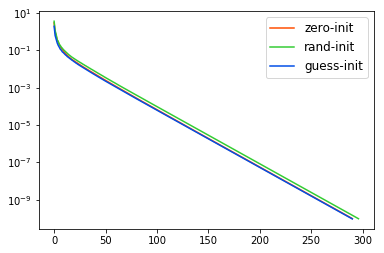
\includegraphics[width=0.4\linewidth]{../output/error.png}
      \label{fig-convergence}
  \end{subfigure}
  \begin{subfigure}
      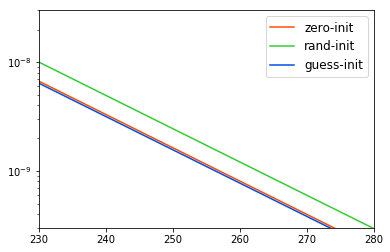
\includegraphics[width=0.4\linewidth]{../output/error-magnified.png}
      \label{fig-convergence-magnified}
  \end{subfigure}
  \caption{Convergence curve of iterative solver. Horizontal axes indicates iteration cycle number. Vertical axes is the maximum value of difference in result for each step.}
\end{figure}

It can be seen that for all three cases, the convergence is satisfying, and guessed initial value is slightly better than zero initial value, which is then better than random initial value. The result is in accordance with the expectation.

Time consumption is very close for three different cases, with guessed initial value slightly faster and random initial value slightly slower. The time consumption is too short to be measured accurately with the \texttt{std::clock()} method, therefore we get 10 to 20 ms for the measurements. However, for the number of iterations depends on the setting of Debye length, this result could be varied, especially when we have a large Debye length (which means the problem is more close to a classical electrostatic equilibrium problem). For time consumption is expected to grow in $O(N)$, for a production problem with the size of $100\times 100\times 20$, this might still only cost around 500 ms to 1 s for the same Debye length.

Memory allocated in this procedure is hard to track with the in-program tracking method, as the memory requirement is small, which is expected to be only a cost on an auxiliary field occupying $20 \times 20\times 10\times 8/10^3\approx 32$ KB. The monitoring function in the program does not show any difference before and during calling of the iterative solver, it might be possible that the solver uses some deprecated memory (reallocated) from the previously called direct solver. The memory allocation for a production problem is still considerably small, for the size of array still grows in $O(N)$, and that will lead to around 1.6 MB for a $100\times 100\times 20$ problem.

\section{Solver Comparison}

Followed is a figure comparing the solutions from direct solver (on the left) and iterative solver (on the right) with the spatial frame $k=5$. It could be seen from the figures that these results are reasonably close to each other.

\begin{figure}[H]
  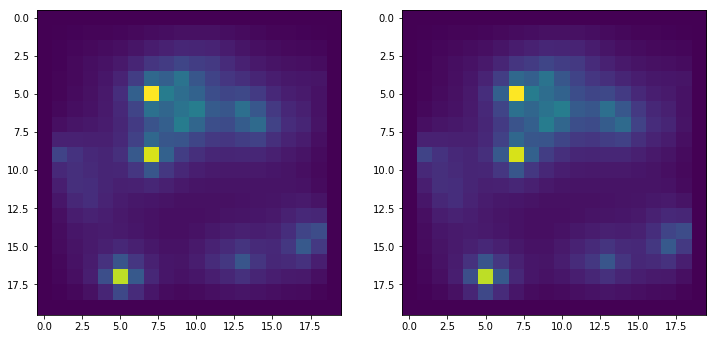
\includegraphics[width=\linewidth]{../output/testcase.png}
  \caption{Comparison between result from direct solver (left) and iterative solver (right).}
  \label{fig-testcase}
\end{figure}

For this certain problem, it is obvious that iterative solver outperforms on both time and memory consumptions. As in real simulations, systems with hundreds of grid points on each dimension are commonly seen, it would be better to use iterative solver compared to the direct solver. However, it could also be seen that the iterative efficiency and accuracy both depend on Debye length ($\lambda_D$) and the requested iteration error limit, with the first one out of manual control, and the second one in need of times of trials. Therefore, although consumption of this method is lower, it might be more tricky to get the satisfying answer via this approach, especially when Debye length is considerably large.

For production problems, they are very likely to be constrained by time consumption of direct solver on first run, which grows as a speed of $O(N^3)$. Therefore before the memory exhausts, it is very likely that the computation time becomes unacceptable. For iterative solver, the major constraint is time (iteration cycle numbers), for the memory consumption is of the same order of magnitude of the consumption for saving an input field. To make the solvers parallel, the partial-pivoting LU-decomposition method might need modifications in order to run on different cores or even nodes.

\section{Discussion and Conclusions}

In this report, we have discussed the physical problem to be solved, the method of discretization, the structure of the matrices/vectors to be constructed, and two different kinds of sequential solvers applied to solving of the problem. We have analyzed and compared the performance of the solvers, leading to the result that Jacobi iterative solver would be a better choice for this certain problem on time and spatial consumptions.

For direct solver, we have seen that matrix decomposition is the most time-consuming part, and the back-solving takes much shorter time for problems with a large size. Therefore it is better than Gauss elimination method in the case we need to solve this equation for many times. For Jacobi iterative solver, we have proved its speed is satisfying, and process makes it compatible for parallel computations since there is no modification on the original array (current step) when carrying out computation on array of the next step.

Real production problem is often of a even larger size, and the most important thing is the rapid growth of time consumption for direct solver, though spatial occupation is still considerably large. For iterative solver, the memory consumption is adequate, therefore the major problem might then lie in the number of cycles in the iteration process.


\newpage
\begin{appendices}

\section{Acknowledgements}

The bracket notation in calling of the matrix element and the stream output operator of matrix are inspired by the grammar from linear algebra template header library named Eigen (\texttt{http://eigen.tuxfamily.org}). The author appreciates these notations making debugging a more concise process.

The method of in-program memory monitoring is inspired from an answer from "Stackoverflow"

(\texttt{https://stackoverflow.com/questions/63166/how-to-determine-cpu-and-memory-consumption-
from-inside-a-process}), which makes use of \texttt{/proc/self/status}.

\section{Code}

The readers can find the code on our Github page (\texttt{https://github.com/sunnyssk/CSE597-hw1}). The source code is inside of \texttt{src} folder, which contains:

\begin{itemize}
    \item \texttt{matrix.h} - Header for matrix class, providing the matrix computation and LU decomposition functions.
    \item \texttt{matrix.cpp} - Source file containing definitions of matrix operations.
    \item \texttt{debye.h} - Declarations of electrostatic function solvers with Debye shielding.
    \item \texttt{debye.cpp} - Definitions of electrostatic solvers.
    \item \texttt{meminfo.h} - Declarations of functions for memory info output.
    \item \texttt{meminfo.cpp} - Definitions of functions for memory info output.
    \item \texttt{main.cpp} - Main entrance of the program. Calls both the direct and iterative solvers.
\end{itemize}

The compile options are listed in Makefile under root directory. Please follow the compile instructions in \texttt{Readme.md} to get the correct version of program. Make sure you have \texttt{-std=c++11} or larger in the compilation options so that \texttt{nullptr} notation is supported by the compiler. To run the program, specify the input filename after the program's name, in the following form:

\texttt{./bin/main ./input/size.txt}

The input file should contain only one line specifying number of grid points on three dimensions ($n_x$,$n_y$,$n_z$). Please be careful that the direct solver could get slow when all three numbers are larger than 20 (which means, there will be more than around 8000 points in the system).

After running the program, the solution of fields will be saved into output folder. If you would like to keep a record of the on-screen tracking information, please use output reorientation. The reader could run this program on any kind of PSU ACI node with basic gcc support.

\section{Licensing and Publishing}

Used in this report is GNU license. The details could be seen in \texttt{license.txt} in root folder of this report, and a copy of GNU license is also attached. Any usage, modifications and redistributions should follow the guidance of this license.

The code is first published within the Pennsylvania State University - University Park.

\end{appendices}

\bibliographystyle{acm}
\bibliography{progressReport}

\end{spacing}

\end{document}

%%%%%%%%%%%%%%%%%%%%%%%%%%%%%%%%%%%%%%%%%%%%%%%%%%%%%%%%%%%%%}}
